\chapter{Addestrare un modello allo stato dell'arte} % Main chapter title
\label{Capitolo5} % Change X to a consecutive number; for referencing this chapter elsewhere, use \ref{ChapterX}
\def \path {Figures/C5}
%--------------------------------------------------------------------
%	SECTION 1
%--------------------------------------------------------------------
\section{Deep Residual Network}
Menzionata nel Capitolo \ref{Capitolo3} a causa del clamore riscosso per l'incredibilmente bassa percentuale d'errore nella ImageNet Challenge del 2015, la \emph{Deep Residual Network} - o ResNet - è una CNN \emph{molto} profonda presentata da Microsoft Research Asia \parencite{resnet} che ha stravolto tutti i record in classification, detection e localization. 
\\ 
L'architettura è modulare: si basa su un blocco detto \emph{"residual block"} (figura \ref{fig:residual}) che viene ripetuto N volte, prima dell'ultimo strato di classificazione. L'idea dietro a questo blocco viene chiamata \emph{residual learning} e funziona così: 
\begin{enumerate}
\item l'input $x$ va attraverso una serie \texttt{conv-relu-conv} dando in output un certo $F(x)$;
\item a questo viene aggiunto l'input originale: $H(x) = F(x) + x$;
\item $F(x)$ è chiamato residual learning. 
\end{enumerate}\\ 
\begin{figure}[h!]
 \centering
 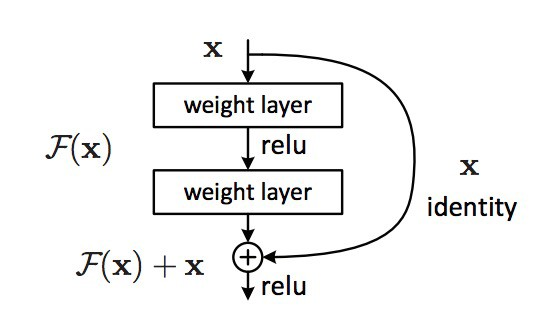
\includegraphics[width=0.6\textwidth]{\path/residual.jpg} 
 \caption{Un "Residual Block", all'input viene aggiunto F(x) che è il residual}
 \label{fig:residual}
\end{figure}

Nelle CNN normalmente si passa direttamente da $x$ a $F(x)$, la quale è una rappresentazione completamente nuova che non mantiene l'informazione dell'input originale. La novità qui, invece, consiste nel mantenere queste informazioni lungo tutta la rete; ogni blocco esegue una sorta di fine-tuning delle informazioni apprese negli strati precedenti, e secondo gli autori è più facile ottimizzare un "residual mapping" anziché un "unreferenced mapping". 
\\
Un esempio della profondità di ResNet è rappresentato in figura \ref{fig:resnet}, dove viene confrontata la versione da 34 strati con la VGG-Network, la rete più profonda che venne presentata 2 anni prima. 
\newpage 

\begin{figure}[h!]
 \centering
 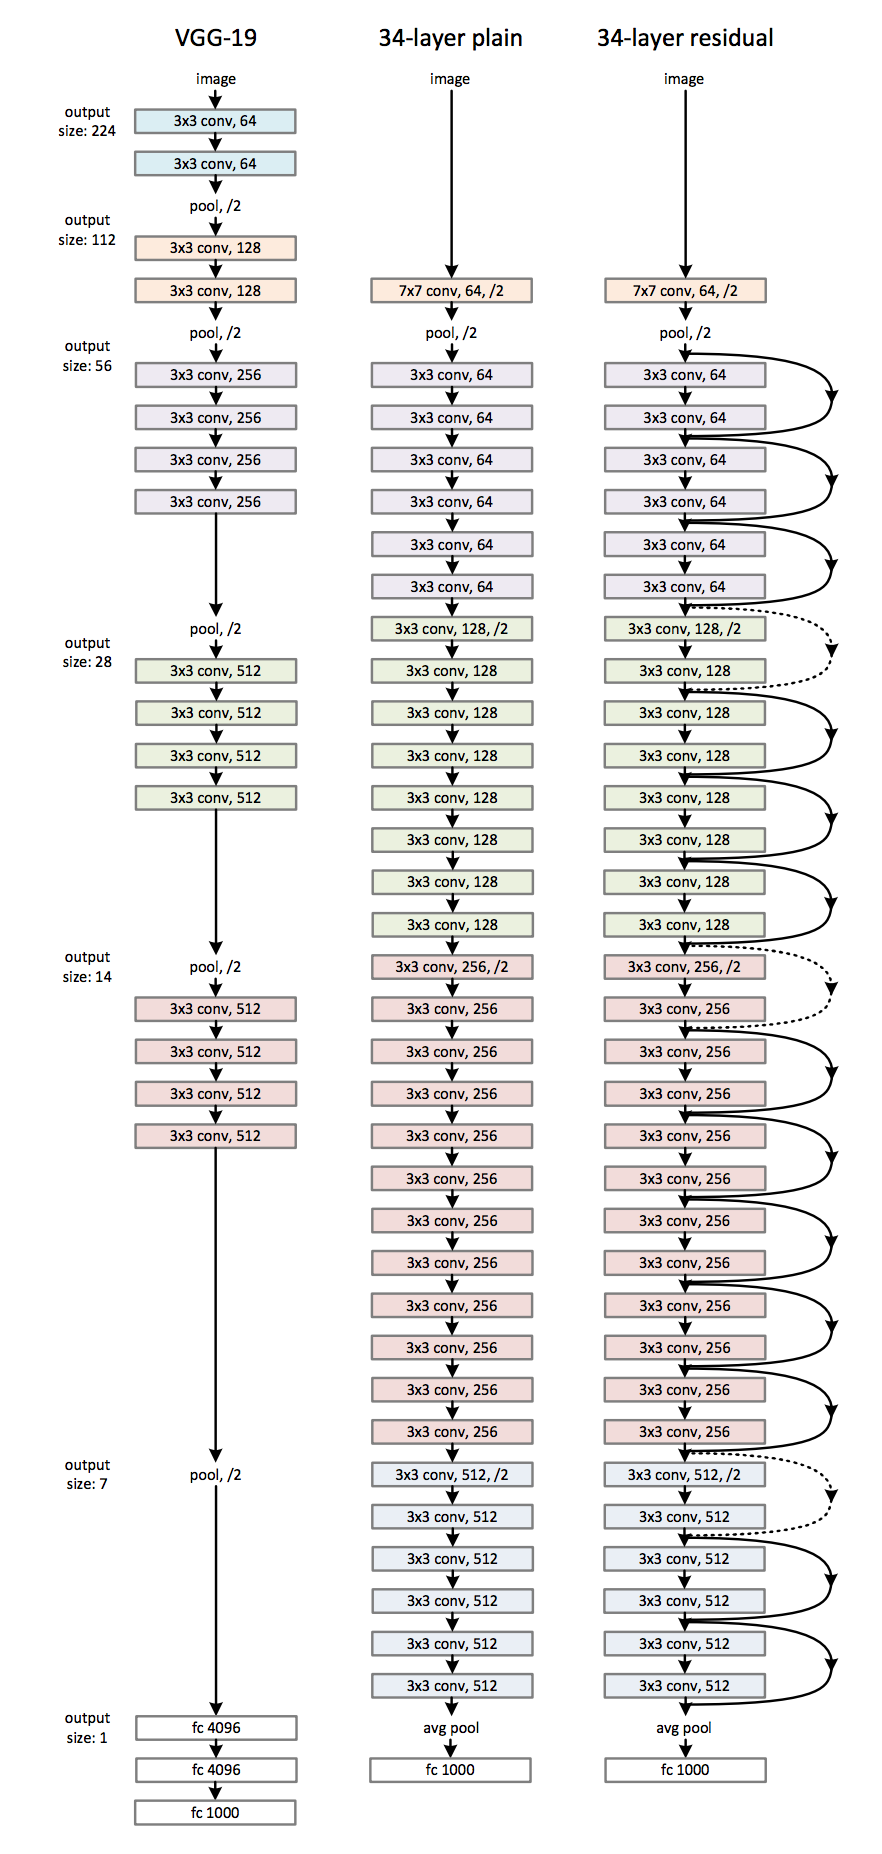
\includegraphics[width=0.7\textwidth]{\path/resnet.png} 
 \caption{Confronto architetture: VGG-Net la più innovativa della competizione ILSVRC 2014, rete classica a 34 strati (centro), Residual Network a 34 strati (sinistra)}
 \label{fig:resnet}
\end{figure}
\bigskip
Un'altra ragione per cui ResNet è stupefacente è che la backpropagation funziona meglio a causa delle somme di ogni layer che distribuiscono la derivata lungo la rete. Inoltre, avere queste scorciatoie che non passano attraverso \texttt{conv-relu} aiuta contro il cruciale problema dei \emph{vanishing gradients}. Quando si usano molti layer uno sull'altro si corre il rischio di non riuscire ad ottimizzare l'apprendimento perché l'errore calcolato con la backprop si perde tra i vari strati e dopo alcuni layer arriva un gradiente nullo che non aiuta nell'apprendimento. Per questa ragione anche, il paper di ResNet è importante: ha dimostrato come poter costruire CNN molto profonde (numero di strati > 100) riuscendo a completare l'apprendimento ed avere inoltre risultati allo stato dell'arte. \\
Tuttavia, altre analisi sul successo di ResNet \parencite{restudy} sostengono il contrario: anche in essa il problema dei vanishing gradients si manifesta dopo \~20 moduli, e quindi la profondità da sola non può essere la caratteristica principale della rete. Suggeriscono invece, che la rete si comporti come un gruppo di "sotto-reti" più piccole che contribuiscono insieme a generare la risposta corretta.\\
È sicuramente un argomento recente e complesso; per ulteriori dettagli si rimanda alla bibliografia. 
 %--------------------------------------------------------------------
%	SECTION 2
%--------------------------------------------------------------------
\section{Implementazione di ResNet di Facebook}
L'implementazione di ResNet è decisamente complessa ma fortunatamente nella community si rilasciano spesso le implementazioni dei modelli più popolari per stimolare i ricercatori a riprodurre gli esperimenti e migliorare sempre di più lo stato dell'arte. A questo proposito Facebook ha rilasciato il codice per diversi modelli di ResNet da 18-34-50-101-152-200 strati. \\
Nei seguenti snippet, vi è l'implementazione della scorciatoia identità e del residual block: 

\begin{lstlisting}[language={[5.2]Lua}]
-- The shortcut layer is either identity or 1x1 convolution
   local function shortcut(nInputPlane, nOutputPlane, stride)
      local useConv = shortcutType == 'C' or
         (shortcutType == 'B' and nInputPlane ~= nOutputPlane)
      if useConv then
         -- 1x1 convolution
         return nn.Sequential()
            :add(Convolution(nInputPlane, nOutputPlane, 1, 1, stride, stride))
            :add(SBatchNorm(nOutputPlane))
      elseif nInputPlane ~= nOutputPlane then
         -- Strided, zero-padded identity shortcut
         return nn.Sequential()
            :add(nn.SpatialAveragePooling(1, 1, stride, stride))
            :add(nn.Concat(2)
               :add(nn.Identity())
               :add(nn.MulConstant(0)))
      else
         return nn.Identity()
      end
   end

   -- The basic residual layer block for 18 and 34 layer network, and the
   -- CIFAR networks
   local function basicblock(n, stride)
      local nInputPlane = iChannels
      iChannels = n

      local s = nn.Sequential()
      s:add(Convolution(nInputPlane,n,3,3,stride,stride,1,1))
      s:add(SBatchNorm(n))
      s:add(ReLU(true))
      s:add(Convolution(n,n,3,3,1,1,1,1))
      s:add(SBatchNorm(n))

      return nn.Sequential()
         :add(nn.ConcatTable()
            :add(s)
            :add(shortcut(nInputPlane, n, stride)))
         :add(nn.CAddTable(true))
         :add(ReLU(true))
   end
\end{lstlisting}
 
Microsoft ha addestrato ResNet per circa 3 settimane su 8 GPU di ultima generazione. Data l'evidente mancanza di hardware opportuno per un'"impresa" del genera si è deciso di utilizzare il modello più piccolo, quello a 18 strati. In apprendice \ref{AppendixB} è mostrata una rappresentazione testuale del modello, ove se ne può apprezzare la complessità e lunghezza. 


%--------------------------------------------------------------------
%	SECTION 3
%--------------------------------------------------------------------
\section{Addestramento su CIFAR}
Si è addestrato il modello ResNet-18 su CIFAR10 per circa 160 epoche. I risultati sul training e validation set sono presentati rispettivamente in figura e figura. Sull'asse X vi sono le epoch di training, sull'asse Y la percentuale di errore. 
\\
La rete da in uscita le 10 classi più probabili; con top1 s'intende quando la classe corretta è la prima più probabile mentre con top5 quando la classe corretta è tra le prime 5 più probabili. \\
\begin{figure}[h!]
 \centering
 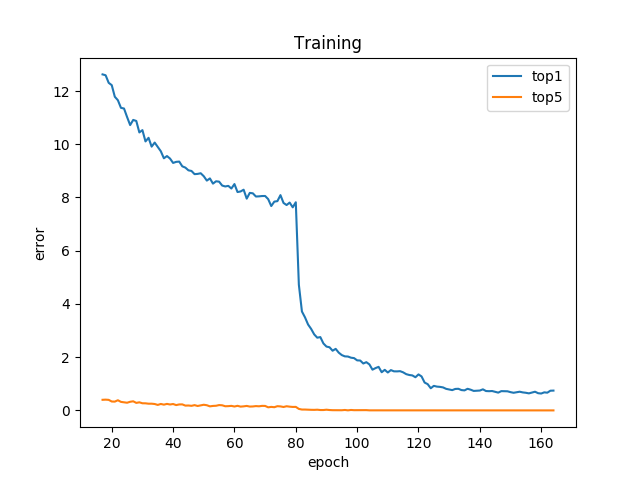
\includegraphics[width=1.0\textwidth]{\path/ResNet-Cifar10-Train.png} 
 \caption{Top-1 e Top-5 training accuracy di ResNet sul dataset CIFAR10}
 \label{fig:res-train}
\end{figure}

\begin{figure}[h!]
 \centering
 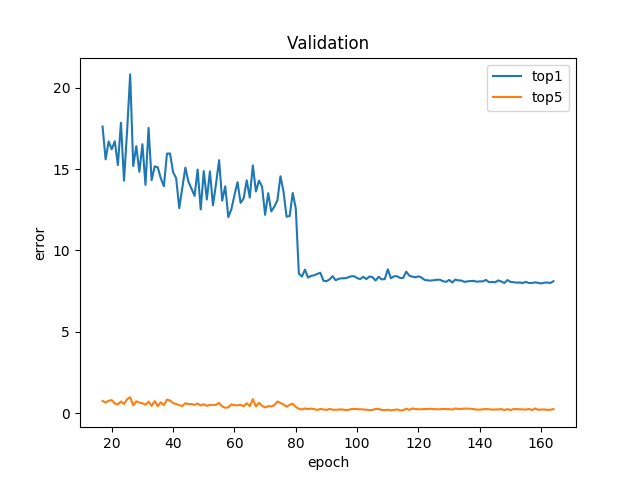
\includegraphics[width=1.0\textwidth]{\path/ResNet-Cifar10-Val.png} 
 \caption{Top-1 e Top-5 validation accuracy di ResNet sul dataset CIFAR10}
 \label{fig:res-val}
\end{figure}

\section{LeNet vs ResNet: confronto}
Nel Capitolo \ref{Capitolo4} si è addestrato uno dei primi modelli di CNN sullo stesso dataset, CIFAR10. La superiorità di ResNet è evidente, raggiunge un'accuratezza di circa il 92-93\% laddove LeNet arrivava appena ad un 73\%. \\
Questo è dovuto a diversi elementi, ma sicuramente è una riprova del fatto che aumentando il numero di layer di convoluzione si aumenta la ricchezza della rappresentazione delle features delle immagini in ingresso e di conseguenza aumenta la capacità della rete di astrarre e "comprendere" molto meglio le informazioni nelle immagini. \\
Ogni anno le architetture delle reti subiscono variazioni e vengono introdotte novità dirompenti che generano nuove riflessioni che spingono quest'ambito di ricerca in avanti ad una velocità tale da mantenere il passo con l'industria delle GPU di cui hanno bisogno per essere  realizzate. 



